This section discussing the working principle of the charging and discharging of the receiving circuit. According to the manufacturer specification $i_r \leq 400 $ mA , which enforces the limit for the system to function properly.
As can be seen in figure \ref{fig:rec_des}, the super capacitor $C_s$ has a very low series resistance of $0.07 \Omega$ compared to $R_L = 65 \Omega$. Therefore we can claim that $i_c \approx i_r$ during charging. If the $i_r(t)$ is not constant, but dependent on time, the capacitor charging is governed by the equation \ref{eq:cap}
\begin{equation}\label{eq:cap}
 V_c = V_{reg} \left(1 - e^{\frac{-t}{R_cC}}\right)
\end{equation}
where $R_c$ is the series limiting resistance of the receiver circuit whose value depends on the maximum value of $i_r$. $C$ is the total capacitance of the supercapacitor which in our case $C_s = 5 $ Farads. $R_c$ can be chosen using $R_c = \frac { V_{reg}}{i_r} $ for a maximum allowed $i_r = 400$ mA which gives us $R_c = 12.5 \Omega$

\begin{figure}[h!]
\centering
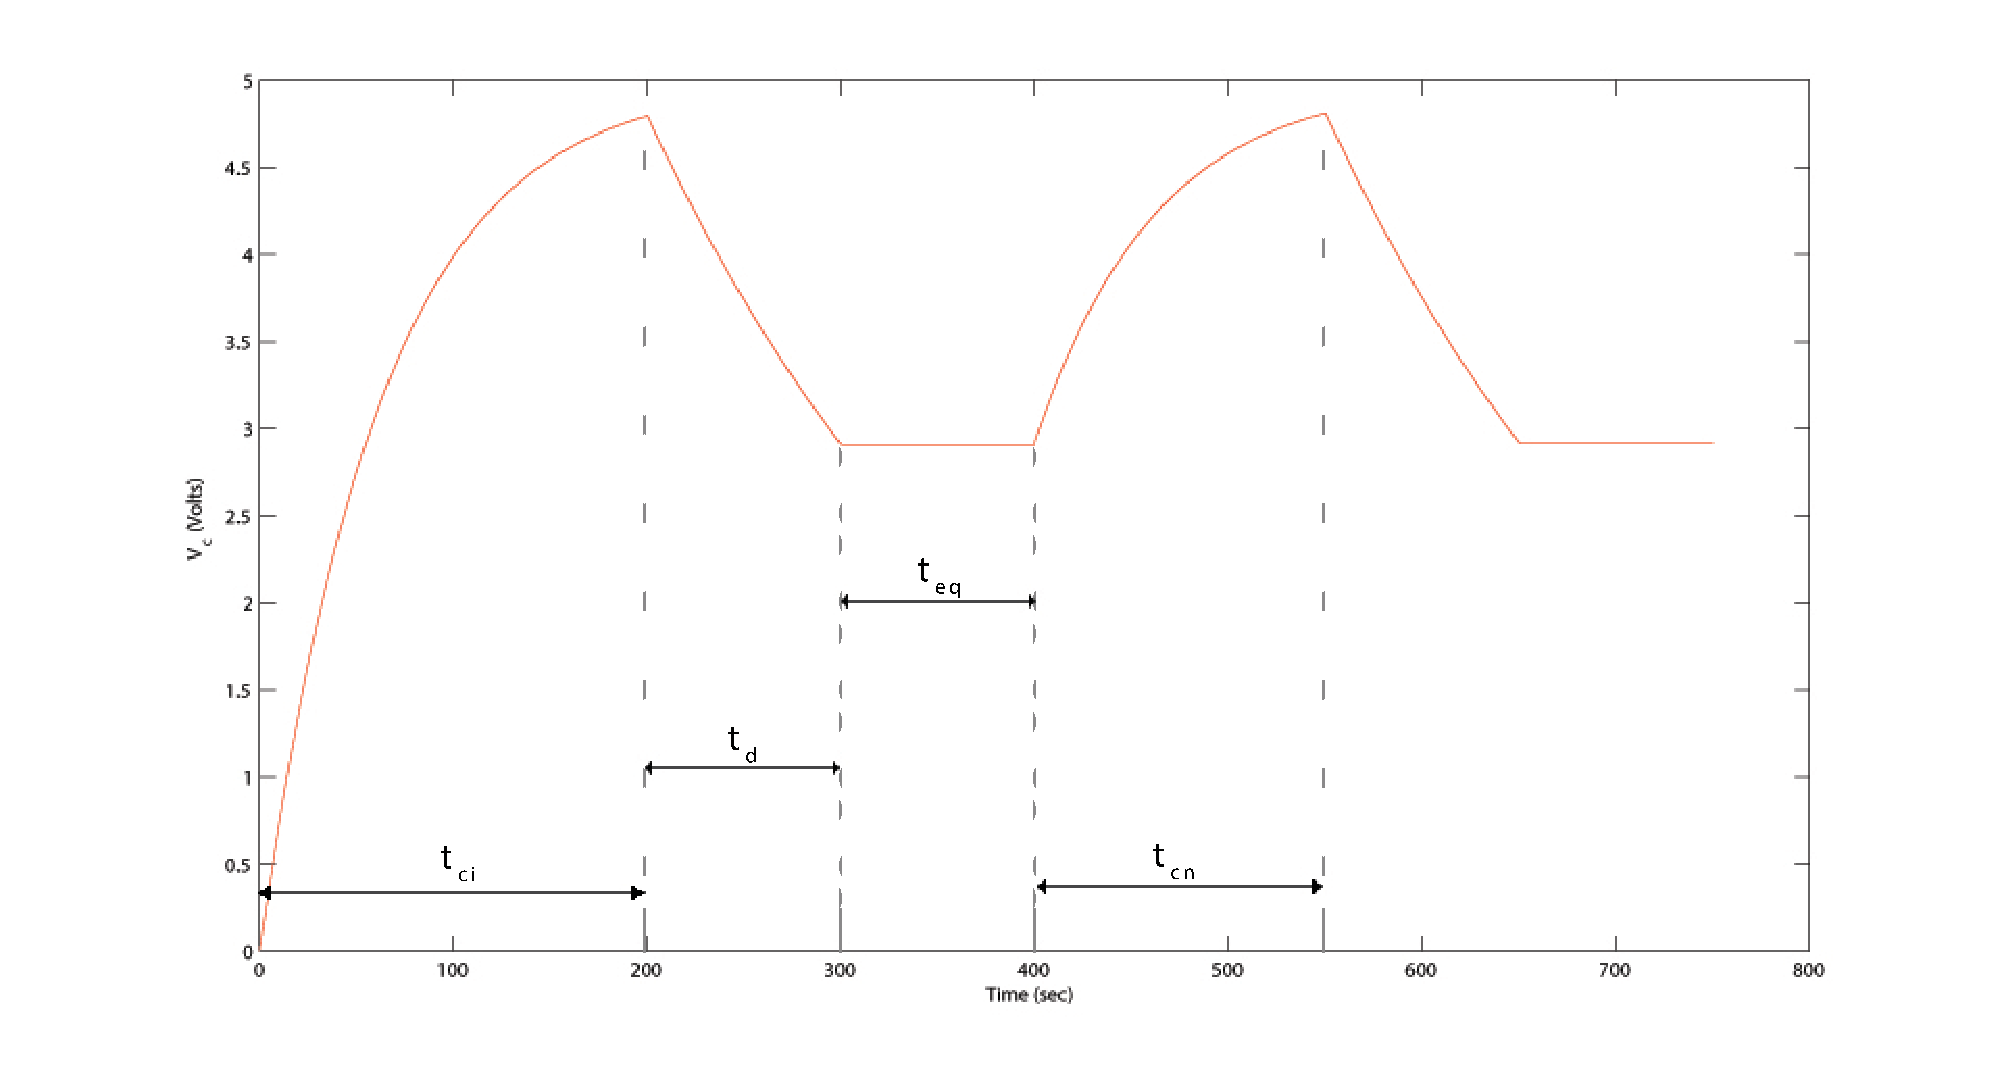
\includegraphics[width=1\textwidth]{cd_cycle.pdf}
\caption{Charging profile of the super capacitor }
\label{fig:ch_profile}
\end{figure}

Figure \ref{fig:ch_profile} displays the charging, discharging and idle profile of the supercapacitor during system operation. In the initial charging cycle $t_{ci}$, $C_s$ is charged using $i_r(t)$ following equation \ref{eq:cap}. During the discharge cycle $t_d$, the $i_r(t) = 0$ and the discharge current is supplied in the form of $i_b$ and $i_L$. Finally during the equilibrium cycle $t_{eq}$ the voltage is reduced to equal the battery voltage ($V_l = 3$ V) such that no current flows between the battery and the supercapacitor and $i_b = 0$. At this stage only the battery's charge is used to power the LED. At last during the second charge cycle $t_{c2}$, the capacitor starts charging from an equilibrium voltage instead of 0 and is charged to $V_{reg}$ untill the discharge cycle starts again. From the above figure we were able to determine appropriate values for the voltage limits as discussed in Section \ref{sec:states}.We choose $V_{max}$ = 3,2V, $V_{full}$ = 3,0V and the starving limit $V_{starving}$ = 2,4V. These values can also be found in the code in the appendix. 
